\documentclass[10pt, a4paper]{article}
\usepackage{preamble}

\title{Discrete Mathematics}
\author{}
\date{January 2025}

\begin{document}

\maketitle

\newpage

\section{Flows and Matchings}

\begin{definition}
    Let $V$ be a finite set,
    the vertices,
    containing two special
    (distinct)
    elements $s$
    (the source)
    and $t$
    (the sink).
    Suppose for every ordered pair $u, v \in V$ we have a capacity $c_{uv}$,
    which is a non-negative integer;
    denote the set of capacities by $C = \{c_{uv}\,:\,u, v \in V\}$.
    We call $(V, C)$ a capacitated network.
\end{definition}

If we have some resource we want to move from the source $s$ to the sink $t$.
We have unlimited resource to transport,
we are limited by the fact that we must route the resource from vertex to vertex is bounded by the capacity $c_{uv}$.
If $c_{uv} = 0$,
we cannot move anything directly from $u$ to $v$,
however there may be an indirect route.

\textbf{Application examples}:

Water flows through pipes,
or a river network,
linking the vertices of $V$.
Our capacity of the river or pipe is the volume of water which can pass through per unit time.

In a road network built on the cities located at vertices of $V$,
traffic can get from city $s$ to city $t$.
The capacity of the road would be how many cars can travel the route per unit time.


We should look at directed graph.

\begin{definition}
    Given a capacitated network $(V, C)$,
    let $E$ be the set of directed edges $E = \{(u, v)\,:\, u, v \in V, c_{uv} > 0\}$.
    Then $G = (V, E)$ is the directed graph representing the available routes on vertices $V$ given capacities $C$.
\end{definition}

Usually we write $uv$ for $(u, v)$.

For convenience,
we will assume:
\begin{enumerate}[label = (\roman*)]
    \item our directed graph has no loops,
    meaning that we suppose that $c_{uu} = 0$ for all $u \in V$;

    \item there's a directed path from $s$ to $t$,
    meaning a sequence of vertices $v_0, \dotsc, v_k \in V$ such that $s = v_0$,
    $t = v_k$,
    $v_{i - 1}v_i \in E$ and for each $1 \leq i \leq k$.
\end{enumerate}

\begin{definition}
    A flow $F$ over the network $(V, C)$ is a set of non-negative integers,
    the flow values,
    $F = \{f_{uv}\,:\, u, v \in V\}$,
    satisfying:
    \begin{enumerate}[label = (\roman*)]
        \item for all $u, v \in V$,
        one has $f_{uv} \leq c_{uv}$,
        i.e.,
        the flow along a directed edge cannot exceed its capacity;

        \item at each vertex $v$ other than $s$ or $t$,
        the sum of the flow values on edges arriving at $v$ is equal to the sum of the flow values on edges leaving $v$.
    \end{enumerate}
\end{definition}


\begin{example}
    Explain why the second condition in the definition of a flow can be expressed as
    \[
    \sum_{u \in V}f_{uv} - \sum_{u \in V}f_{vu} = 0,\qquad\text{provided $v \notin \{s, t\}$}.
    \]
    What if $v = s$ or $t$?
    Define $\Phi_{in}(F) = \sum_{v \in V}f_{sv} - \sum_{u \in V}f_{us}$
    (the net amount of flow generated by the source)
    and $\Phi_{out}(F) = \sum_{u \in V}f_{ut} - \sum_{v \in V}f_{tv}$
    (the net amount of flow drained at the sink).
    
    \begin{solution}
        We have $V = \{v_1, \dotsc, v_N\}$
        (\textit{Note:
        we are including the source $s$ and sink $t$ in the set of vertices $V$})
        \[
        \sum_{u \in V}f_{uv} - \sum_{u \in V}f_{vu} = 0
        \]
        \[
        \sum_{u \in V}f_{uv}  = f_{v_1v} + f_{v_2v} + \dotsc + f_{v_nv} = \text{the flow into $v$}
        \]
        \[
        \sum_{u \in V}f_{vu}  = f_{vv_1} + f_{vv_2} + \dotsc + f_{vv_n} = \text{the flow out of $v$}.
        \]
        So the flow into $v$ equals the flow out of $v$.
    \end{solution}
\end{example}

\begin{example}
    Explain why $\sum_{u, v \in V}f_{uv} = \sum_{u, v \in V}f_{vu}$
    (this uses neither of the properties of a flow).
    Use this together with the formula in the previous exercise to show that $\Phi_{in}(F) = \Phi_{out}(F)$.

    \begin{solution}
        By the cases $u, v \in V \setminus \{s, t\}$.
        We can apply the previous repeatedly for any $v \in V \setminus \{s, t\}$.

        Now for $u, v \in \{s, t\}$.
        Flow into $s$ is $0$,
        $f_{vs} = 0$ for all $v \in V$ because there are no loops and the source only goes out.
        $\sum_{v \in V}f_{sv} = \sum_{v \in V}f_{vt}$
        (the flow out of $s$ to $v$ is equal to the flow from $v$ to $t$)
        because the flow into any vertex equals the flow going out of any vertex.
        $f_{tv} = 0$ for all $v \in V$ since there's no flow going out of $t$.
    \end{solution}
\end{example}

\begin{center}
    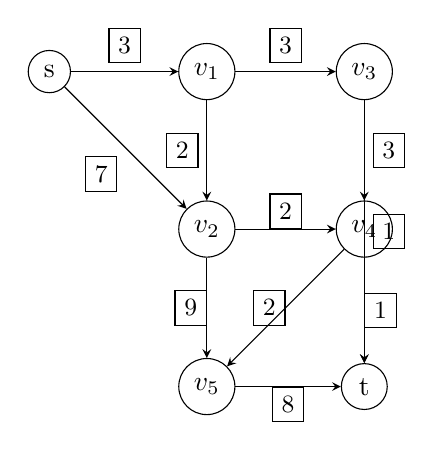
\begin{tikzpicture}[>=stealth, node distance=2cm, every node/.style={draw, circle}]
        % Nodes
        \node (s) {s};
        \node[right of=s] (v1) {$v_1$};
        \node[right of=v1] (v3) {$v_3$};
        \node[below of=v1] (v2) {$v_2$};
        \node[right of=v2] (v4) {$v_4$};
        \node[below of=v2] (v5) {$v_5$};
        \node[right of=v5] (t) {t};

        % Edges
        \draw[->] (s) -- (v1) node[midway, above, rectangle, minimum size = 10pt, yshift = 3pt] {\small 3};
        \draw[->] (s) -- (v2) node[midway, below left, yshift = -3pt, xshift = -3pt, rectangle] {\small 7};
        \draw[->] (v1) -- (v2) node[midway, left, rectangle, xshift = -3pt] {\small 2};
        \draw[->] (v1) -- (v3) node[midway, above, rectangle, yshift = 3pt] {\small 3};
        \draw[->] (v2) -- (v5) node[midway, left, rectangle] {\small 9};
        \draw[->] (v2) -- (v4) node[midway, above, rectangle] {\small 2};
        \draw[->] (v3) -- (v4) node[midway, right, rectangle, xshift = 3pt] {\small 3};
        \draw[->] (v3) -- (t) node[midway, right, rectangle, xshift = 3pt] {\small 1};
        \draw[->] (v4) -- (v5) node[midway, left, rectangle] {\small 2};
        \draw[->] (v4) -- (t) node[midway, right, rectangle] {\small 1};
        \draw[->] (v5) -- (t) node[midway, below, rectangle] {\small 8};
    \end{tikzpicture}
\end{center}

\end{document}